%!TEX root = ../DevaramaniS-[RnD-MT]Report.tex

\chapter{Design and Implementation} 

The adaptation of the \textit{Vereshchagin solver} to the kinematic tree structure was presented in previous chapter. The first step in applying this extended solver to mobile robots is to model the robot as a kinematic tree. 

A kinematic tree comprises of interconnected segments (links). A typical kinematic tree description is provided by \hyperref[kdl]{KDL} library. Here, a single segment (KDL::Segment) is described as following~\cite{kinematictreeKDL},

\begin{figure}[h!]
	\begin{center}
		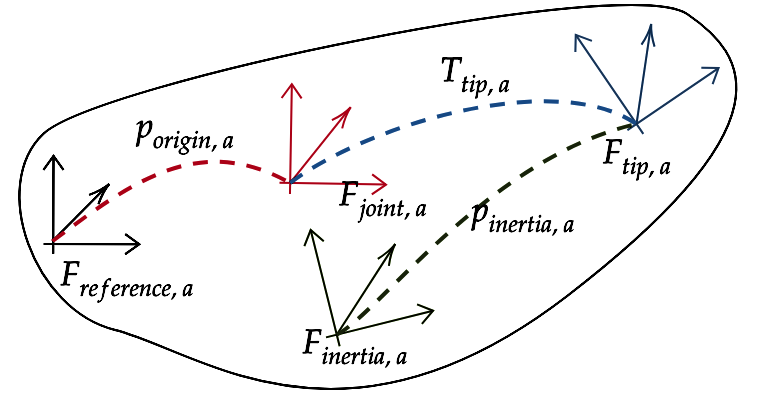
\includegraphics[scale=0.3]{images/segment}
	\end{center}
	\caption{KDL Segment}
	\label{fig:segment}
\end{figure} 

The above figure \ref{fig:segment} represents a KDL segment composing of four frames,
\begin{enumerate}
	\item $F_{reference}$: A \textit{reference} frame (black colored frame) with respect to which other frames are expressed.
	\item $F_{joint}$: A one DOF \textit{joint} frame (red) expressed about joint axis. The orientation of the frame is same as $F_{reference}$ and translation is given by $p_{origin, a}$.
	\item $F_{inertia}$: A \textit{rotational inertia frame} (green) expressed with respect to \textit{tip frame} and $p_{inertia, a}$ is the translation vector. The frame is defined under KDL::RigidBodyInertia library.
	\item $F_{tip}$: Frame attached at the tip of a segment. As seen in the figure \ref{fig:segment}, $F_{tip, a}$ is defined with respect to joint frame (blue) and transformation is given by $T_{tip, a}$ (by default: $T_{tip, a}$ is identity transformation). 
\end{enumerate}

A Kinematic tree is simply a composition of these KDL segments. An example is shown in the below figure (\ref{fig:kinematic-tree}) which describes a \textit{Kinematic tree} with two branches~\cite{kinematictreeKDL}. According to the convention, the joint frame of the succeeding segment is attached to tip frame of the preceding segment. Hence, the tip frames acts as the reference frame for the succeeding segments ($F_{tip, a} = F_{reference, b} = F_{reference, c}$). Similarly, the representation can be extended to multiple chains or interconnected segments. 

\begin{figure}[h!]
	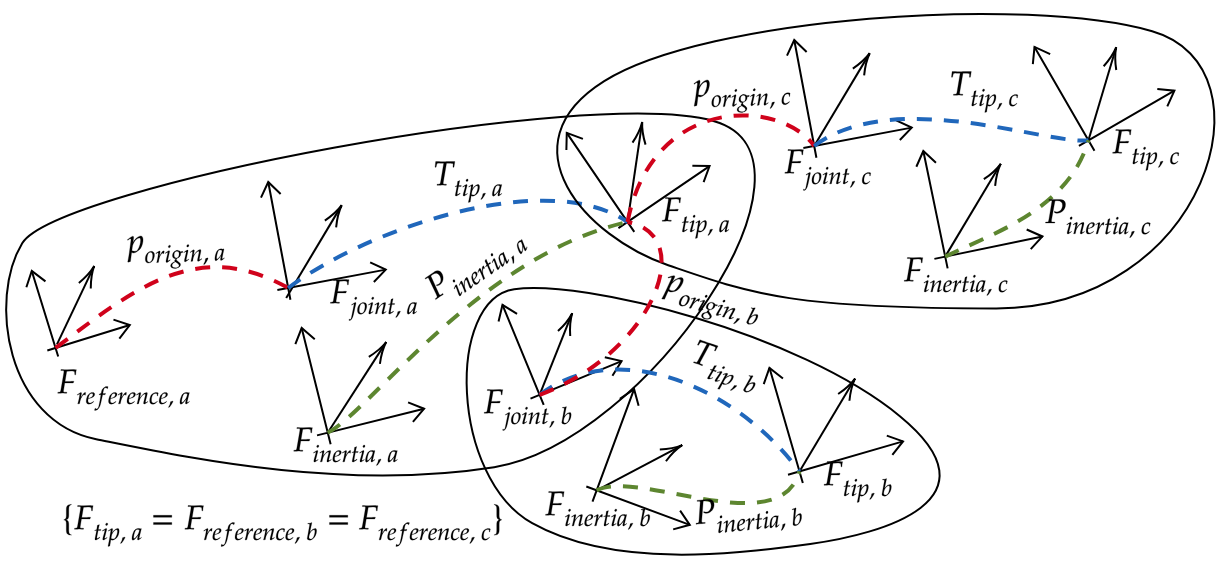
\includegraphics[scale=0.35]{images/kinematic-tree}
	\caption{Kinematic tree representation in KDL}
		\label{fig:kinematic-tree}
\end{figure}


\section{Design details}
A mobile robot can be modeled as a kinematic tree with base of the robot as root of the tree and wheels as end-effectors. The following section provides detailed description software design and simulation of the approach. The robot platform used to model as kinematic tree structure is MPO-700 (figure \ref{fig:MPO-700})~\cite{MPO700}. 

\begin{figure}[h!]
	\centering
	
	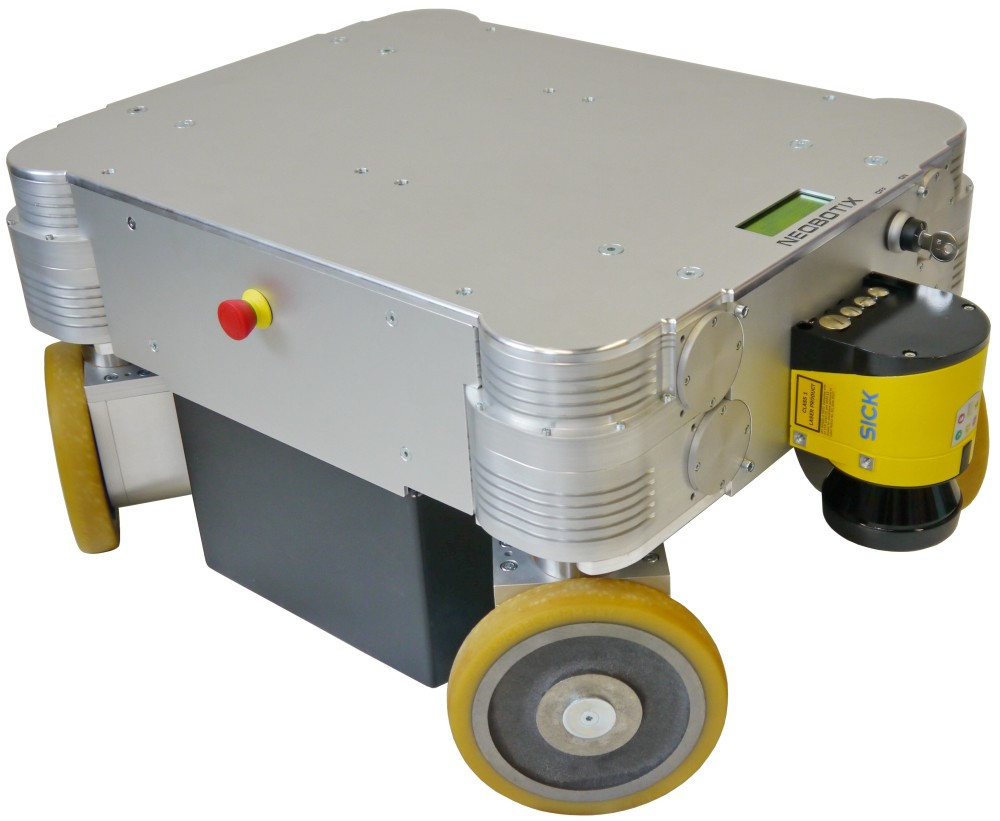
\includegraphics[scale=0.4]{images/mp0700}
	\caption{MPO-700 Neobotix}
	\label{fig:MPO-700}
\end{figure}

\subsection{Robot Specifications}
MPO-700 is an omni-directional base employed in high-end service robots~\cite{Neobotix-homepage}. The base features four \textit{Neobotix omnidirectional modules} that enables smooth motion in X-Y directions. When compared to other robot bases with omnidirectional drive kinematics, the MPO-700 has great maneuverability, steadiness, high stability and compact~\cite{Neobotix-homepage}. Hence, it is used in wide range of applications. One of the popular platform built based of MPO-700 is \textit{Care-O-bot} 3 developed by Fraunhofer IPA\footnote{Fraunhofer IPA - \url{http://www.ipa.fraunhofer.de}}. 

For modeling the MPO-700, the base is defined as root of the kinematic tree. Further, the segments individually defined as KDL::Segment, are connected to the \textit{root}. Using the technical dimensions from the MPO-700 operating manual, the four frames (figure \ref{fig:segment}) of each of the segments are modeled. 

\begin{figure}[h!]
	\centering
	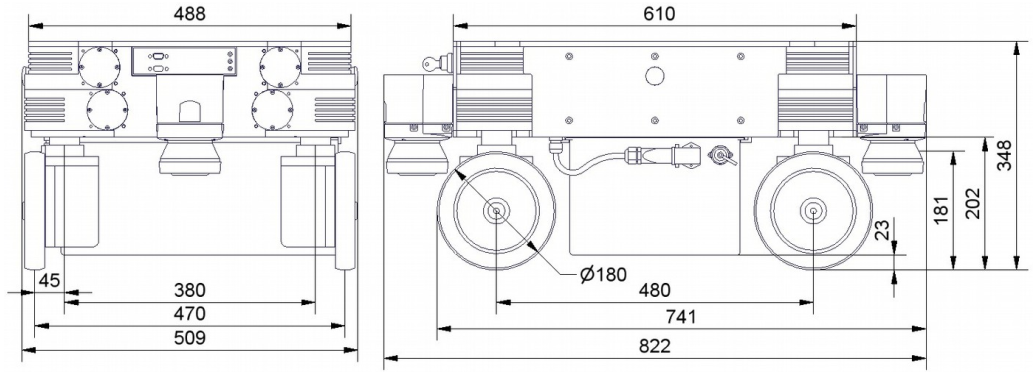
\includegraphics[scale=0.4]{images/technicaldata}
	\caption{MPO-700 dimensions (source:~\cite{MPO700-Datasheet})}
	\label{fig:Technicaldata}
\end{figure}

\begin{figure}[h!]
	\centering
	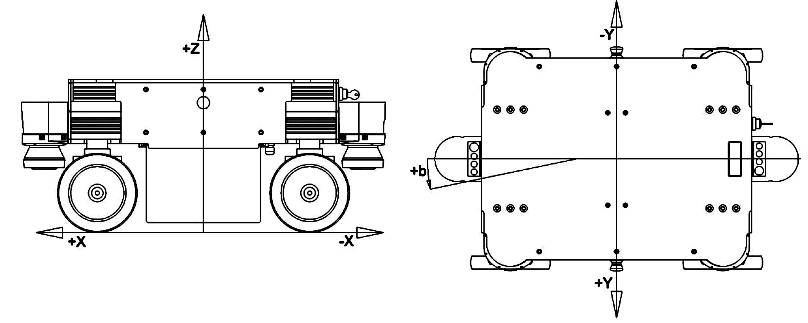
\includegraphics[scale=0.4]{images/coordinate}
	\caption{MPO-700 Coordinate system convention (source:~\cite{MPO700})}
	\label{fig:coordinate}
\end{figure}
To define a physical link as KDL::Segment, The required information to describe a physical link as a KDL::Segment are, 



 To this root, further segments of type KDL::Segment are connected. According to the dimensions available in the Operating manual~\cite{MPO700}, the 




It has four Castor wheels that enables the base to move along X-Y directions. By default, the wheels are considered to be oriented inwards by $45^0$ (as seen in figure \ref{fig:MPO-700}). 


